
\phantomsection
\pagestyle{plain}

\begingroup

\let\clearpage\relax
\let\cleardoublepage\relax
\let\cleardoublepage\relax

\interlude{Environmental Governance in India}\label{box:clearances}

\noindent Vijay Ramesh\textsuperscript{1}, \textbf{Pratik R. Gupte}, and Mridula M. Paul\textsuperscript{2}

\graffito{
	\textsuperscript{1} Columbia University, USA.
	
	\medskip
	
	\textsuperscript{2} Ashoka Trust for Research in Ecology and the Environment, India.
}

\medskip

\noindent {{$\Delta$}} {\footnotesize This box is adapted from an article written in response to the publication of the Draft Environmental Impact Assessment (EIA) Rules, 2020, in India --- only one among a spate of efforts worldwide to use the Covid-19 pandemic as cover for sweeping changes to regulations in environmental policy and civil liberties.
The article appeared online in \textit{Sanctuary Asia}.}

\medskip
\footnotesize

\begin{figure}[h!]
	\centering
	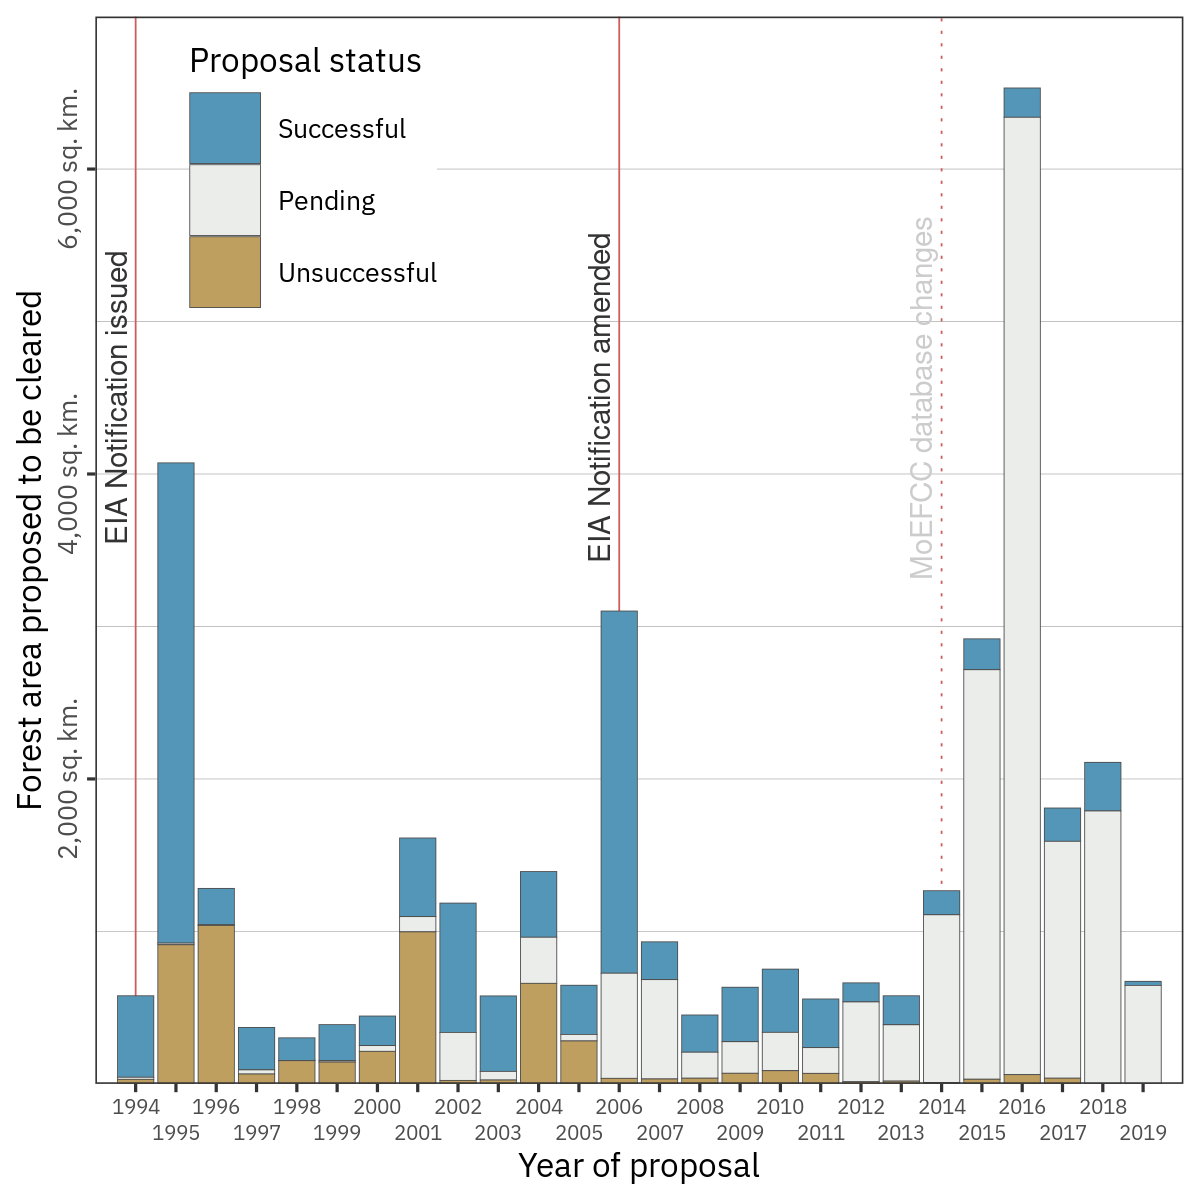
\includegraphics[width=0.7\textwidth]{figures/boxes/clearances.png}
	\caption*{
		\textbf{Forest areas proposed to be cleared since the advent of environmental protections in India.} 
		Forest area (in sq. km.) proposed for clearance over the years 1994 -- 2019, coloured to show the fraction approved (blue), rejected (brown), and pending decision (grey). Projects applied for nearly twice as much area to be cleared in years when or shortly after a new EIA notification was adopted (1995 and 2006), as in other years. Since the approval rate for projects did not differ significantly among years, 1995 and 2006 saw 814\% more forest area approved for clearance than other years.
	}
	\label{fig_box_clearances}
\end{figure}

Environmental Impact Assessments (EIA) are crucial to balance environmental imperatives with economic development.  
In March 2020, the Government of India's Ministry of Environment, Forest and Climate Change (MoEFCC) published a revised draft Environmental Impact Assessment (EIA) Notification, titled Draft EIA 2020, to make the process of granting project approval more standardized and transparent \footnote{``Draft EIA Notification'' (New Delhi, 2020).}. 
Environmentalists nationwide have voiced significant concerns with respect to this draft, citing considerable dilution of existing EIA regulations \footnote{``India's push to relax environmental assessment rules amid pandemic draws criticism.'' Science (2020).}. 

The EIA Notification was initially issued in 1994 \footnote{``The Environmental Impact Assessment Notification'' (S.O.60(E), New Delhi, 1994).}, and further revised by ministerial notification in 2006 \footnote{``Environmental Impact Assessment Notification'' (S.O.1533(E), New Delhi, 2006)}. 
Analysis of MoEFCC forest clearance data \footnote{PARIVESH Portal (available at https://parivesh.nic.in/).} between 1994 and 2019 shows that projects applied for significantly more forest area to be cleared in years when or shortly after a new EIA notification was adopted. 
These years, 1995 and 2006, saw approximately 4,000 sq.km. and approximately 3,000 sq.km. respectively, proposed for clearance, which is nearly twice as much area proposed in other years. 
Further, applications in 1995 and 2006 were just as successful as they were in other years, and thus 814\% more forest area was approved for clearance compared to other years.

Between 1994 and 2013, 70\% of forest area proposed for clearances was approved. 
If this clearance rate were applied to forest clearances pending since 2014, India could see an additional 9,900 sq. km. of forest land cleared, about twice as much as in the preceding twenty years combined. 
Provisions in the Draft EIA Rules, 2020, such as regularisation of environmental safeguards violations, or allowing projects to fence off forest land before the EIA process could cause further forest loss and degradation commensurate with 1995 and 2006. 
MoEFCC must reconsider the Draft EIA Rules, 2020, and strengthen environmental governance if India is to meet national reforestation \footnote{``Bonn Challenge and India: Progress on restoration efforts across states and landscapes.'' IUCN (2018).} and international climate targets \footnote{``India needs to double rate of forest cover expansion to achieve Paris Agreement target''. Mongabay India (2019)}.

%, (available at https://portals.iucn.org/library/sites/library/files/documents/2018-026-En.pdf).
% , (available at https://india.mongabay.com/2019/11/paris-agreement-goals-india-needs-to-double-forest-cover-expansion-rate/).

{ \begin{center} \barfont{-.-} \end{center} }

\endgroup

\afterpage{\nopagecolor}
\pagestyle{scrheadings}
